% 长方体 ABCD-A1B1C1D1 示意，E 在 AB 上，F 在 BC 上；虚线为遮挡棱与内部研究线段
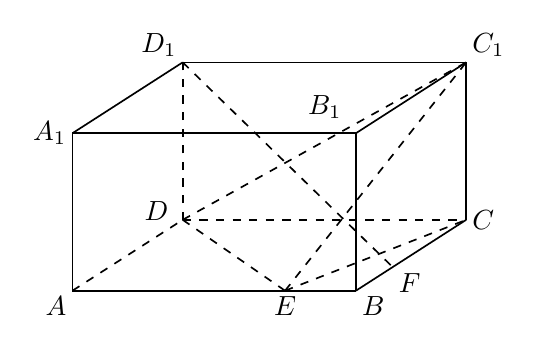
\begin{tikzpicture}[x=1cm,y=1cm,font=\normalsize,
  solidedge/.style={solid,line width=.6pt,draw=black},
  hidedge/.style={dashed,line width=.6pt,draw=black},
  ptlabel/.style={font=\normalsize,inner sep=2pt}]
\coordinate (A) at (0,0);
\coordinate (E) at (2.7000000000,0.0000000000);
\coordinate (B) at (3.6,0);
\coordinate (D) at (1.4,0.9);
\coordinate (C) at (5.0,0.9);
\coordinate (F) at (4.0666666667,0.3000000000);
\coordinate (A1) at (0,2.0);
\coordinate (B1) at (3.6,2.0);
\coordinate (D1) at (1.4,2.9);
\coordinate (C1) at (5.0,2.9);
% 可见轮廓：前面、顶面前沿、左右竖棱、右侧面
\draw[solidedge] (A) -- (E) -- (B);
\draw[solidedge] (B) -- (C);
\draw[solidedge] (C) -- (C1);
\draw[solidedge] (C1) -- (D1);
\draw[solidedge] (D1) -- (A1);
\draw[solidedge] (A1) -- (A);
\draw[solidedge] (A1) -- (B1);
\draw[solidedge] (B1) -- (B);
\draw[solidedge] (B1) -- (C1);

% 遮挡棱
\draw[hidedge] (A) -- (D);
\draw[hidedge] (D) -- (C);
\draw[hidedge] (D) -- (D1);
% 内部研究线段（原图虚线）
\draw[hidedge] (D) -- (E);
\draw[hidedge] (E) -- (C);
\draw[hidedge] (E) -- (C1);
\draw[hidedge] (D) -- (C1);

\draw[hidedge] (D1) -- (F);

\node[ptlabel,below left] at (A) {$A$};
\node[ptlabel,below] at (E) {$E$};
\node[ptlabel,below right] at (B) {$B$};
\node[ptlabel,left,xshift=-3pt,yshift=3pt] at (D) {$D$};
\node[ptlabel,right] at (C) {$C$};
\node[ptlabel,below right] at (F) {$F$};
\node[ptlabel,left] at (A1) {$A_{1}$};
\node[ptlabel,above left=3pt] at (B1) {$B_{1}$};
\node[ptlabel,above left] at (D1) {$D_{1}$};
\node[ptlabel,above right] at (C1) {$C_{1}$};
\end{tikzpicture}
